\section{Results}
\label{sec:results}

To investigate the sensitivity of this search with the current exclusivity cuts 
we use the transverse mass $m_T$ to perform a fit. Figure~\ref{fig:mT}
shows the $m_T$ distributions for the signal and all the backgrounds.
Z+jets and W+jets are estimated by scaling using exclusivity efficiencies obtained 
from data. The assumption here is that the shape change for these samples due to 
the exclusivity cut is not very significant. An investigation on the validity of this 
assumption is an active area of research. 
 
\begin{figure}[!h]
\centering
\begin{tabular}{c}
	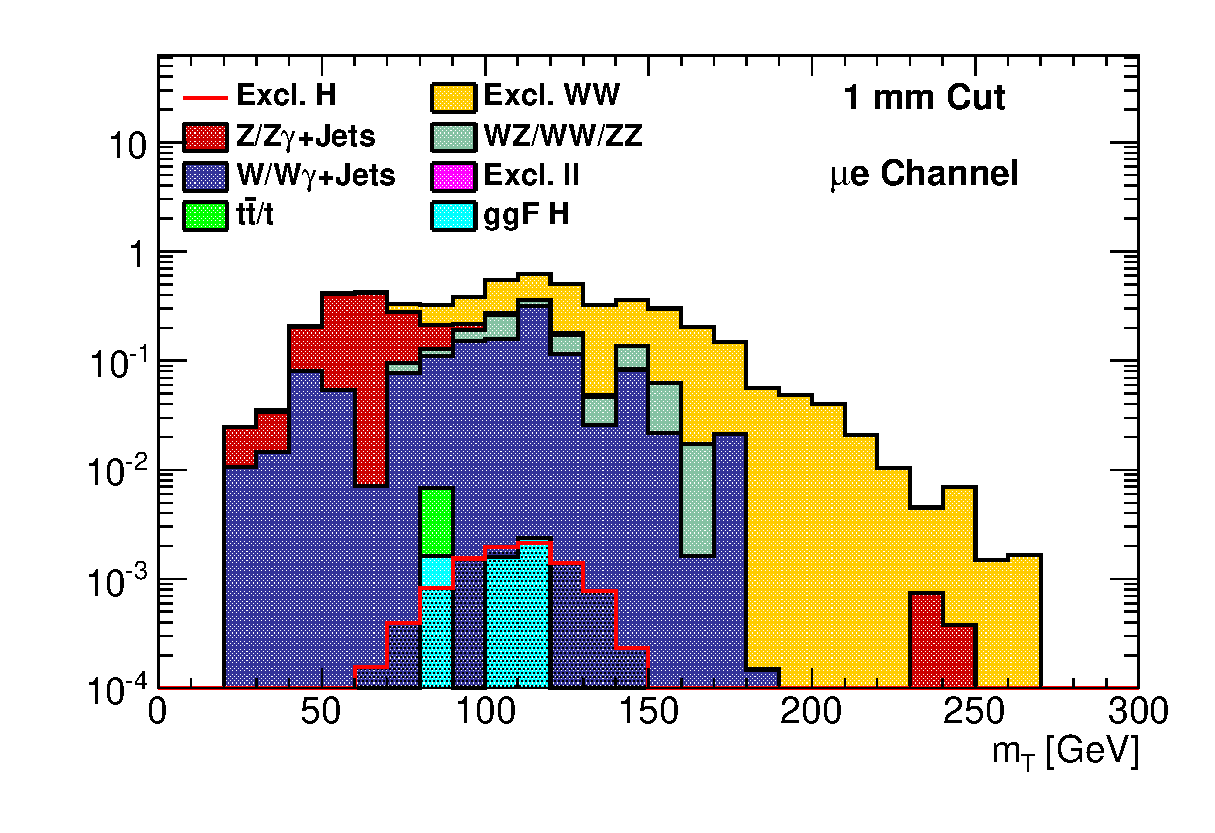
\includegraphics[width=0.5\linewidth]{h_mT_sig_mue.eps}
	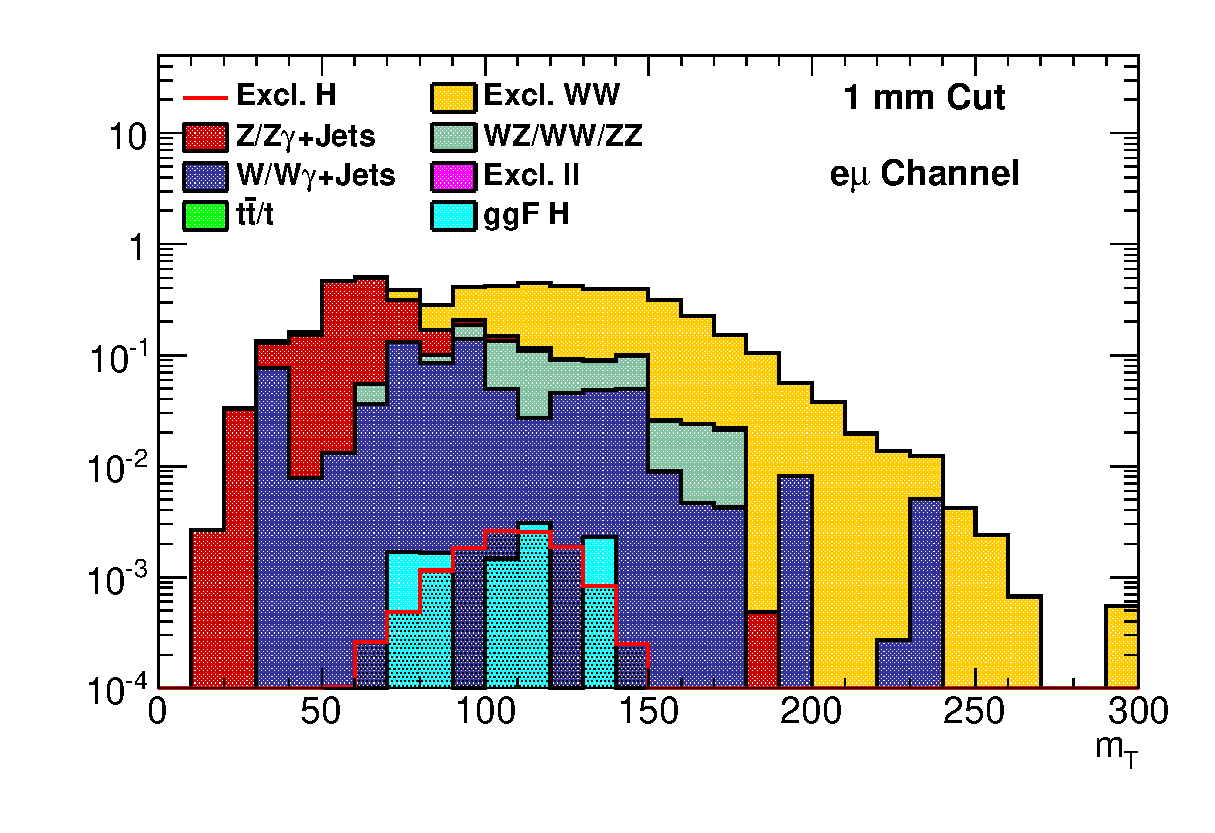
\includegraphics[width=0.5\linewidth]{h_mT_sig_emu.eps}
\end{tabular}
\caption{$m_{T}$ distributions for signal and background. The signal is not part of the stack.}
\label{fig:mT}
\end{figure}

The fit performed in a 1-bin fit for $75<m_T<150\ GeV$. The only systematic uncertainty accounted for 
here is the uncertainty associated with the integrated luminosity. The majority of the uncertainties 
are therefore statistical. Table~\ref{table:limits} shows the limits obtained. 

\begin{table}[!h]
\begin{center}
\begin{tabular}{cc|cccc}
Cut & Limit [pb] & $+1\sigma$ & $+2\sigma$ & $-1\sigma$ & $-2\sigma$ \\
\hline
1 mm & 1.19 & 1.78 & 2.67 & 0.86 & 0.64 \\
\end{tabular}
\end{center}
\caption{Limits set by fitting with $m_T$.}
\label{table:limits}
\end{table}

These limits exclude .... 
